% !TEX TS-program = pdflatex
% !TEX encoding = UTF-8 Unicode

% This is a simple template for a LaTeX document using the "article" class.
% See "book", "report", "letter" for other types of document.

\documentclass[20pt]{article} % use larger type; default would be 10pt

\usepackage[utf8]{inputenc} % set input encoding (not needed with XeLaTeX)

%%% Examples of Article customizations
% These packages are optional, depending whether you want the features they provide.
% See the LaTeX Companion or other references for full information.

%%% PAGE DIMENSIONS
\usepackage{geometry} % to change the page dimensions
\geometry{a4paper} % or letterpaper (US) or a5paper or....
% \geometry{margin=2in} % for example, change the margins to 2 inches all round
% \geometry{landscape} % set up the page for landscape
%   read geometry.pdf for detailed page layout information

\usepackage{graphicx} % support the \includegraphics command and options

% \usepackage[parfill]{parskip} % Activate to begin paragraphs with an empty line rather than an indent

%%% PACKAGES
\usepackage{booktabs} % for much better looking tables
\usepackage{array} % for better arrays (eg matrices) in maths
\usepackage{paralist} % very flexible & customisable lists (eg. enumerate/itemize, etc.)
\usepackage{verbatim} % adds environment for commenting out blocks of text & for better verbatim
%\usepackage{subfig} % make it possible to include more than one captioned figure/table in a single float
\usepackage{mathtools}
\usepackage{graphicx} % supports images in latex
% These packages are all incorporated in the memoir class to one degree or another...

\usepackage{graphicx}
\usepackage{subcaption}

%%% Other stuff
\DeclarePairedDelimiter\ceil{\lceil}{\rceil}
\DeclarePairedDelimiter\floor{\lfloor}{\rfloor}

%%% HEADERS & FOOTERS
\usepackage{fancyhdr} % This should be set AFTER setting up the page geometry
\pagestyle{fancy} % options: empty , plain , fancy
\renewcommand{\headrulewidth}{0pt} % customise the layout...
\lhead{}\chead{}\rhead{}
\lfoot{}\cfoot{\thepage}\rfoot{}

%%% SECTION TITLE APPEARANCE
\usepackage{sectsty}
\allsectionsfont{\sffamily\mdseries\upshape} % (See the fntguide.pdf for font help)
% (This matches ConTeXt defaults)

%%% ToC (table of contents) APPEARANCE
\usepackage[nottoc,notlof,notlot]{tocbibind} % Put the bibliography in the ToC
\usepackage[titles,subfigure]{tocloft} % Alter the style of the Table of Contents
\renewcommand{\cftsecfont}{\rmfamily\mdseries\upshape}
\renewcommand{\cftsecpagefont}{\rmfamily\mdseries\upshape} % No bold!

%%% graphics path


%%% END Article customizations

%%% nice things to keep around
%\begin{figure}[!htbp]
%  	\centering
%   	\begin{subfigure}[p]{0.5\linewidth}
%    	\includegraphics[width=\linewidth]{}
%   	\end{subfigure}
%\end{figure} 

% \noindent\rule{2cm}{0.4pt} 
%%% puts a small horizontal line

% \mathcal{O} 
%%% big O notation

%%% The "real" document content comes below...

\title{Formal Languages Homework 2}
\author{Liam Dillingham}
%\date{} % Activate to display a given date or no date (if empty),
         % otherwise the current date is printed 

\begin{document}
\maketitle

\section{Problem 2.3.2}
Convert to a DFA the following NFA: 
\begin{figure}[!htbp]
  	\centering
   	\begin{subfigure}[p]{0.25\linewidth}
    	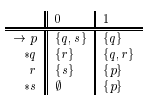
\includegraphics[width=\linewidth]{./figures/HW2fig1.png}
   	\end{subfigure}
\end{figure} \\
\noindent\rule{2cm}{0.4pt} \\
\begin{figure}[!htbp]
  	\centering
   	\begin{subfigure}[p]{1.1\linewidth}
    	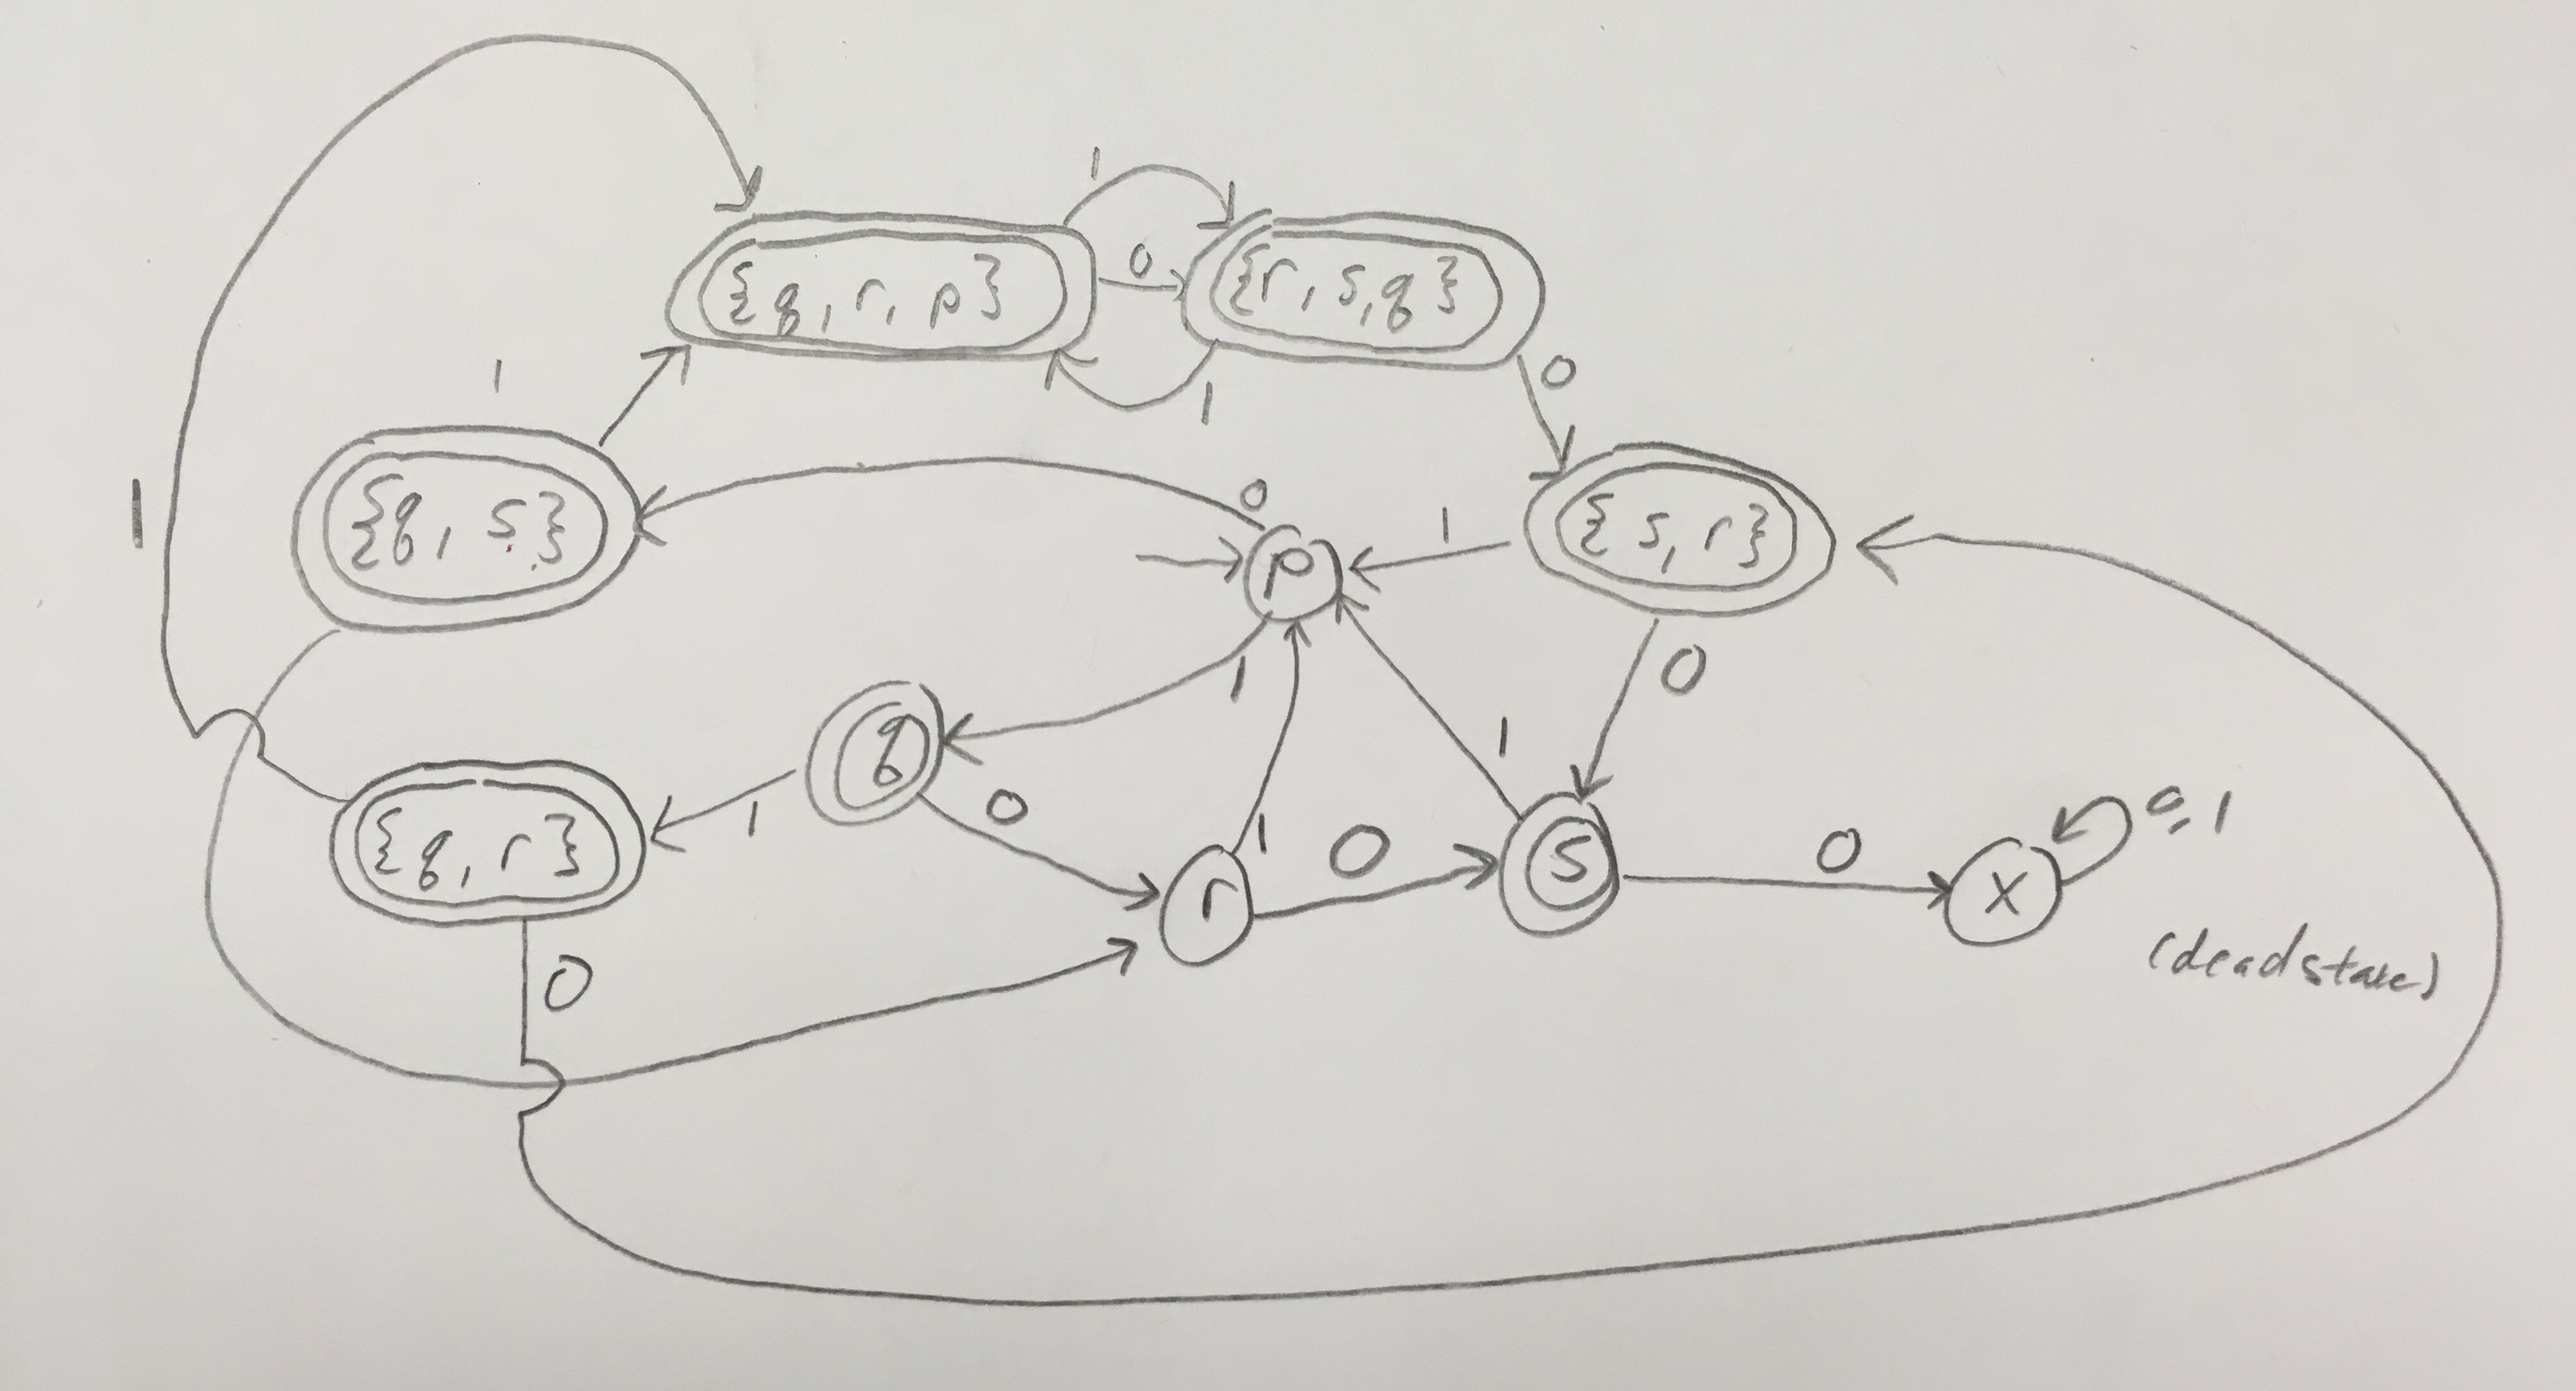
\includegraphics[width=\linewidth]{./figures/h2-1.jpg}
   	\end{subfigure}
\end{figure}


\section{Problem 2.3.3}
Convert the following NFA to a DFA and informally describe the language it accepts. 
\begin{figure}[!htbp]
  	\centering
   	\begin{subfigure}[p]{0.25\linewidth}
    	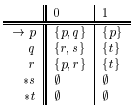
\includegraphics[width=\linewidth]{./figures/HW2fig2.png}
   	\end{subfigure}
\end{figure} \\
\noindent\rule{2cm}{0.4pt} \\
\begin{figure}[!htbp]
  	\centering
   	\begin{subfigure}[p]{0.95\linewidth}
    	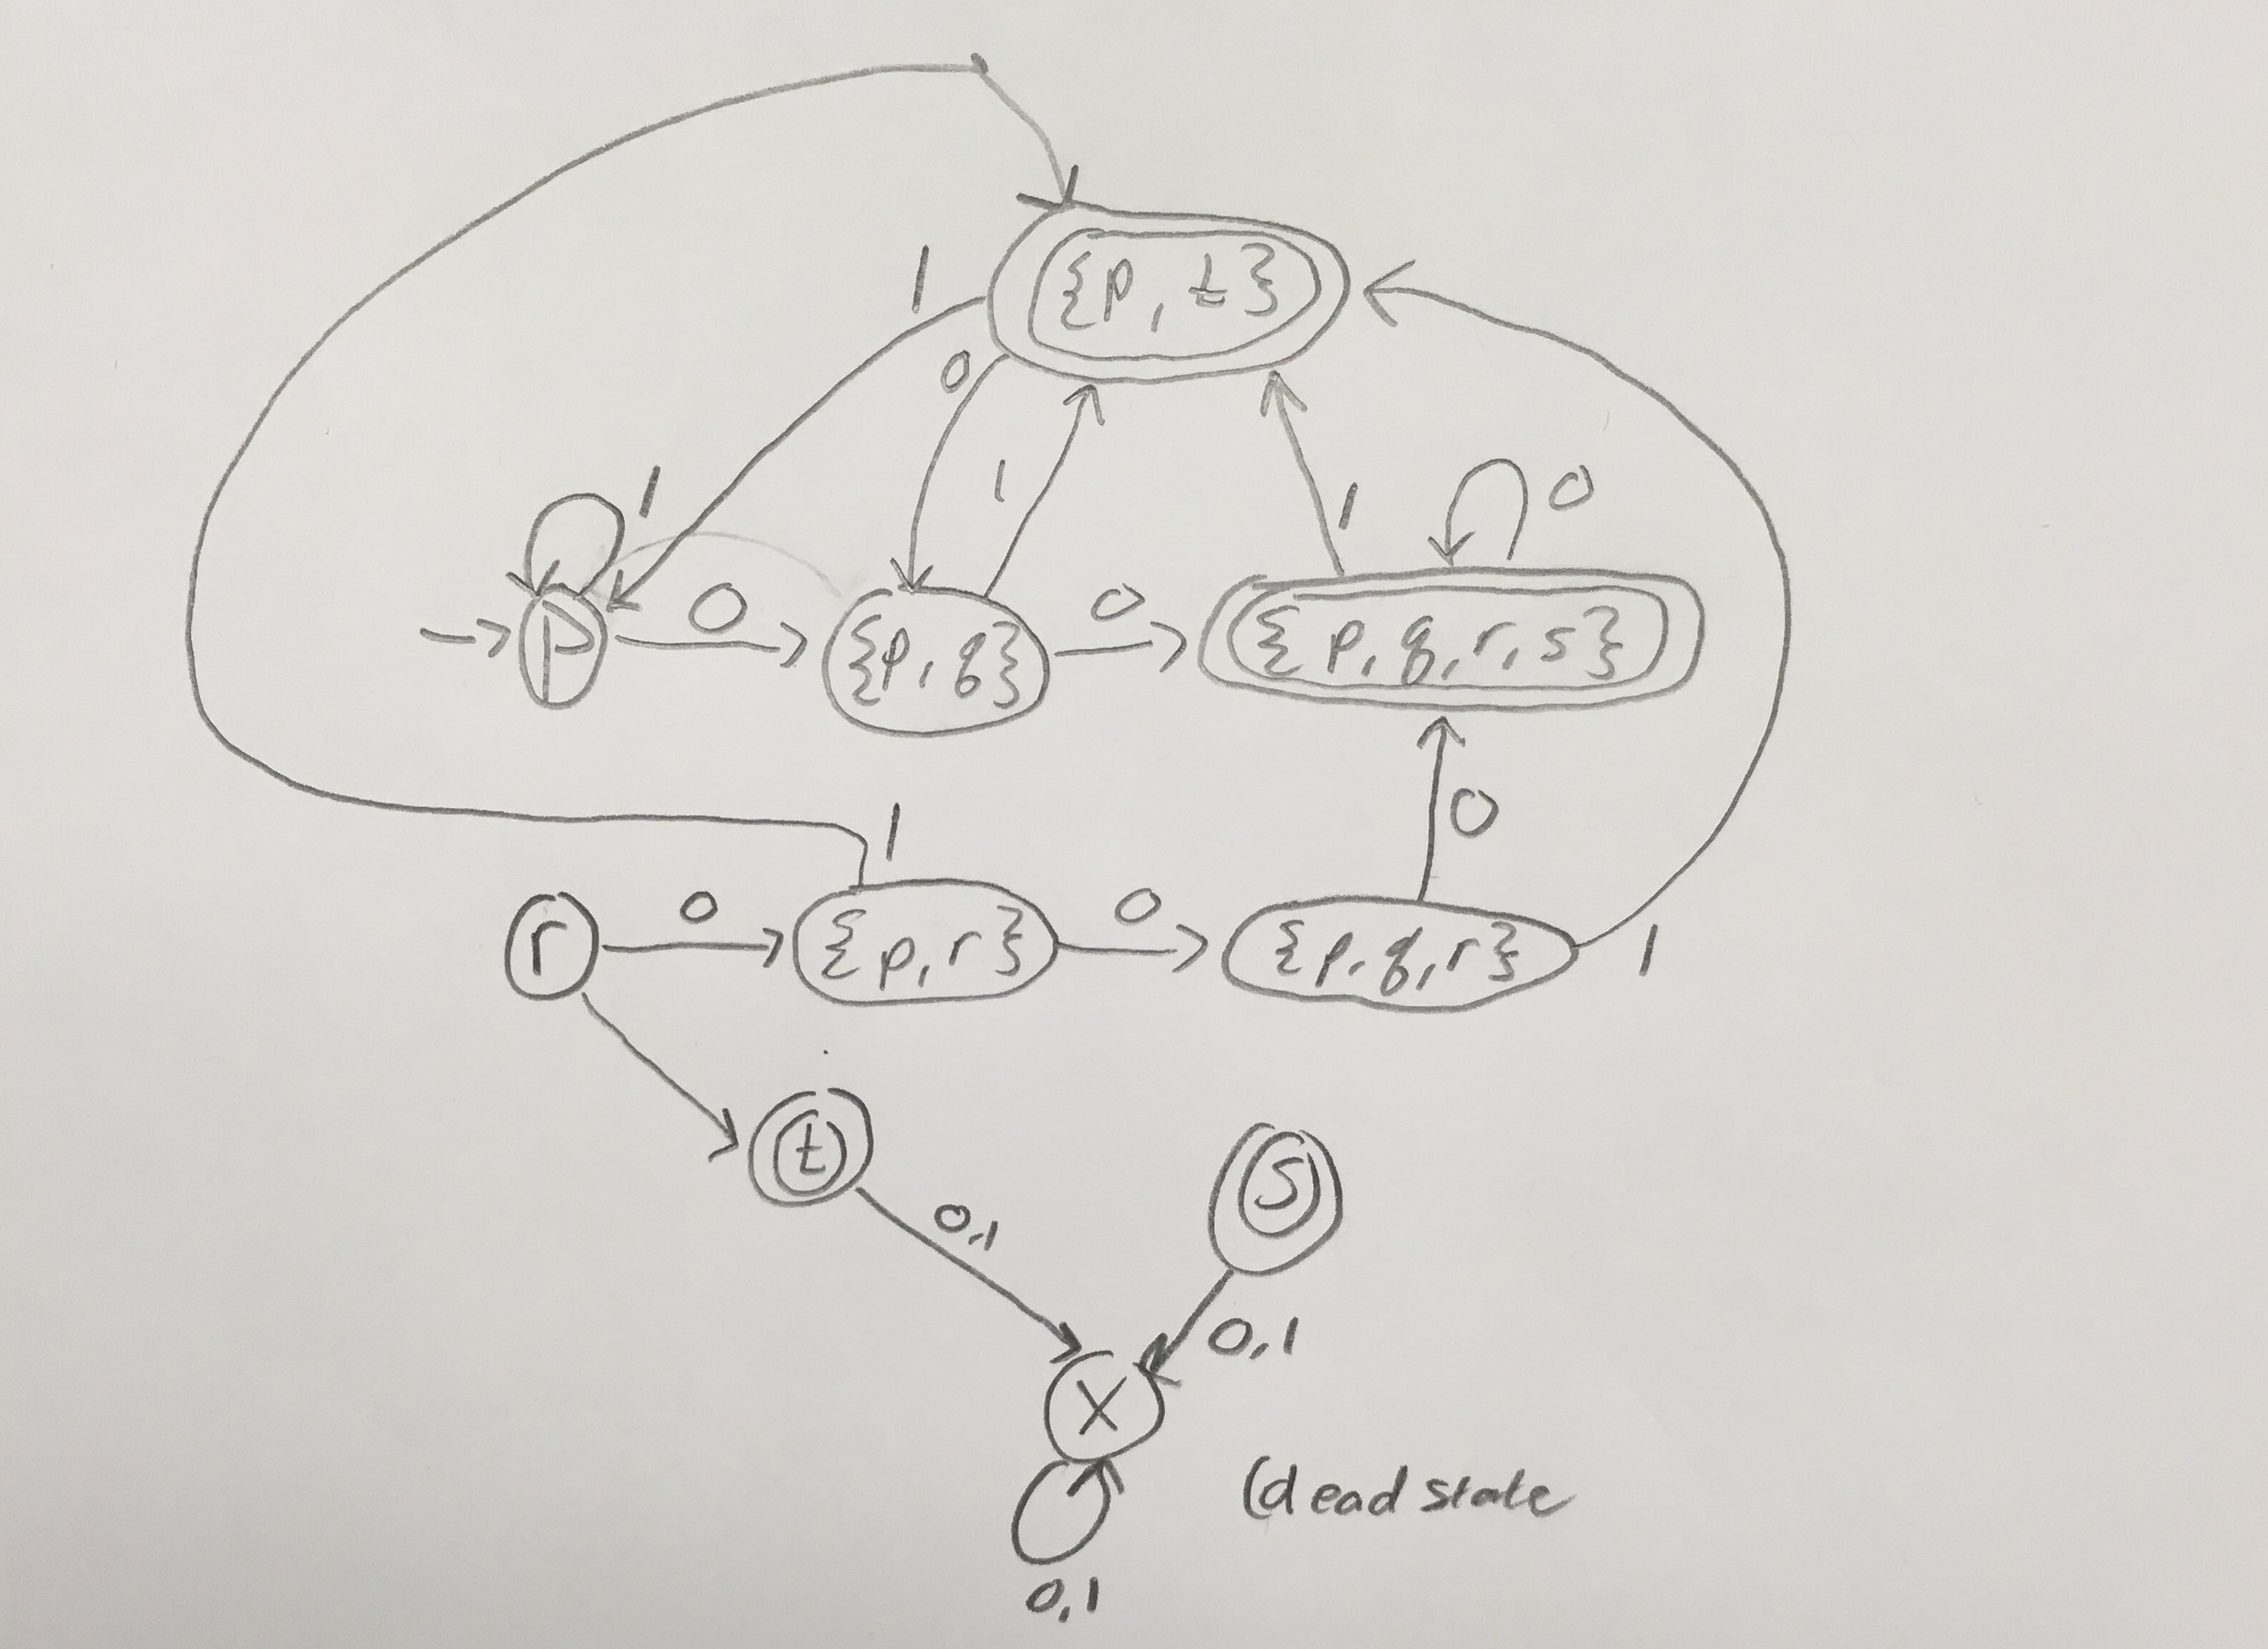
\includegraphics[width=\linewidth]{./figures/h2-2.jpg}
   	\end{subfigure}
\end{figure} \\
The language accepted by the NFA/DFA is all strings ending in $00$, or $01$.

\newpage
\section{Problem 2.3.4} 
Give nondeterministic finite automata to accept the following languages. Try to take advantage of nondeterminism as much as possible
\subsection{a). The set of strings over alphabet $\{0,1,...,9\}$ such that the final digit has appeared before}
\begin{figure}[!htbp]
  	\centering
   	\begin{subfigure}[p]{0.9\linewidth}
    	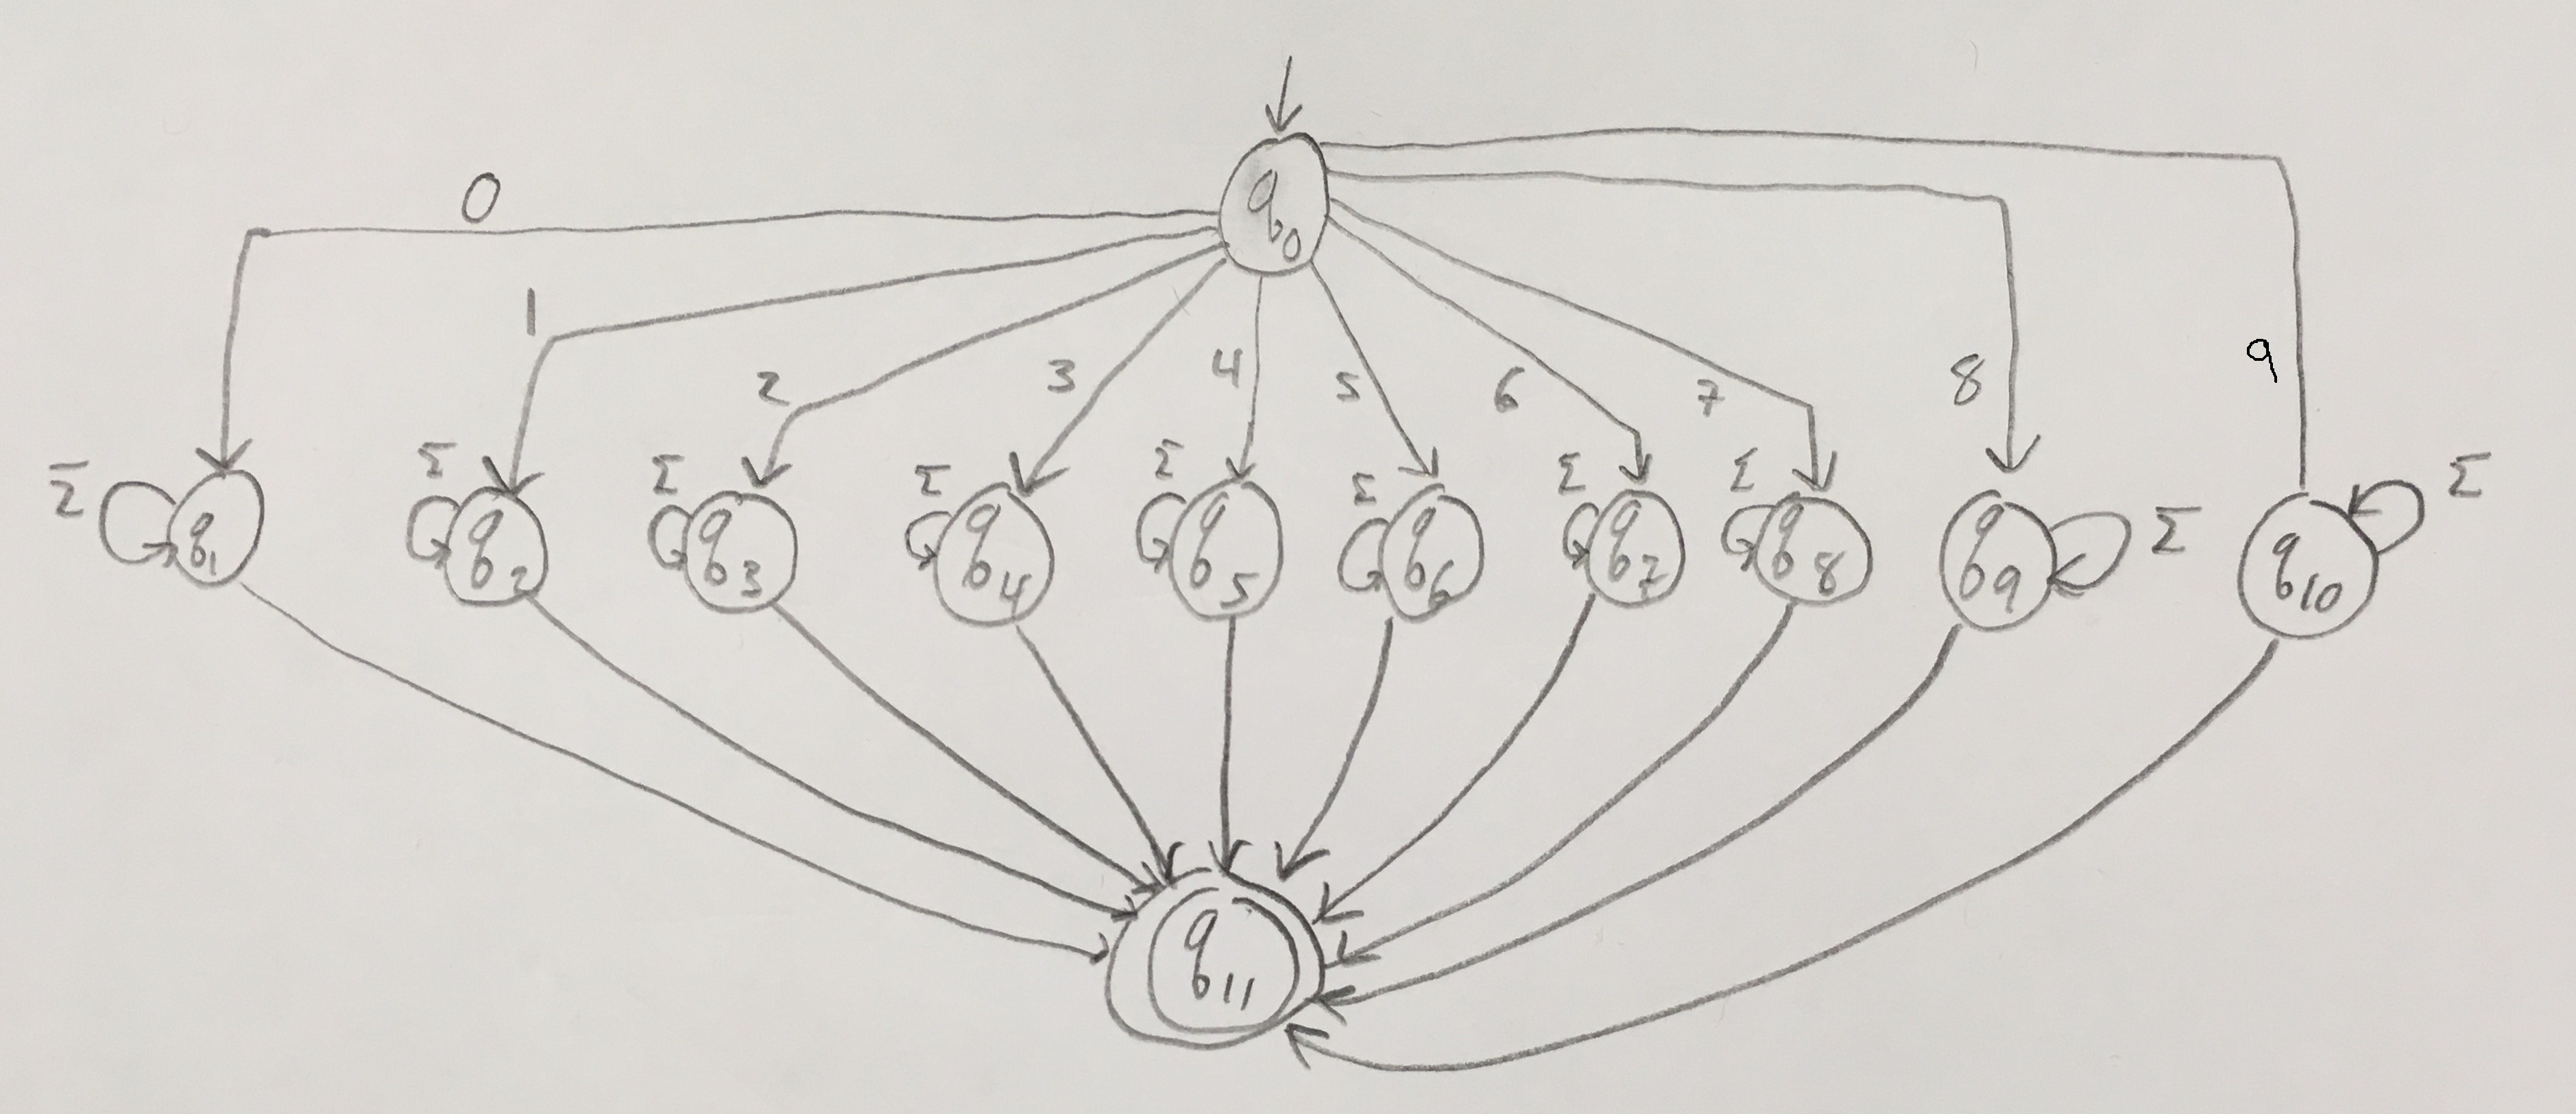
\includegraphics[width=\linewidth]{./figures/h2-3.jpg}
   	\end{subfigure}
\end{figure}
\subsection{b). The set of strings over alphabet $\{0,1,...,9\}$ such that the final digit has not appeared before}
\begin{figure}[!htbp]
  	\centering
   	\begin{subfigure}[p]{0.9\linewidth}
    	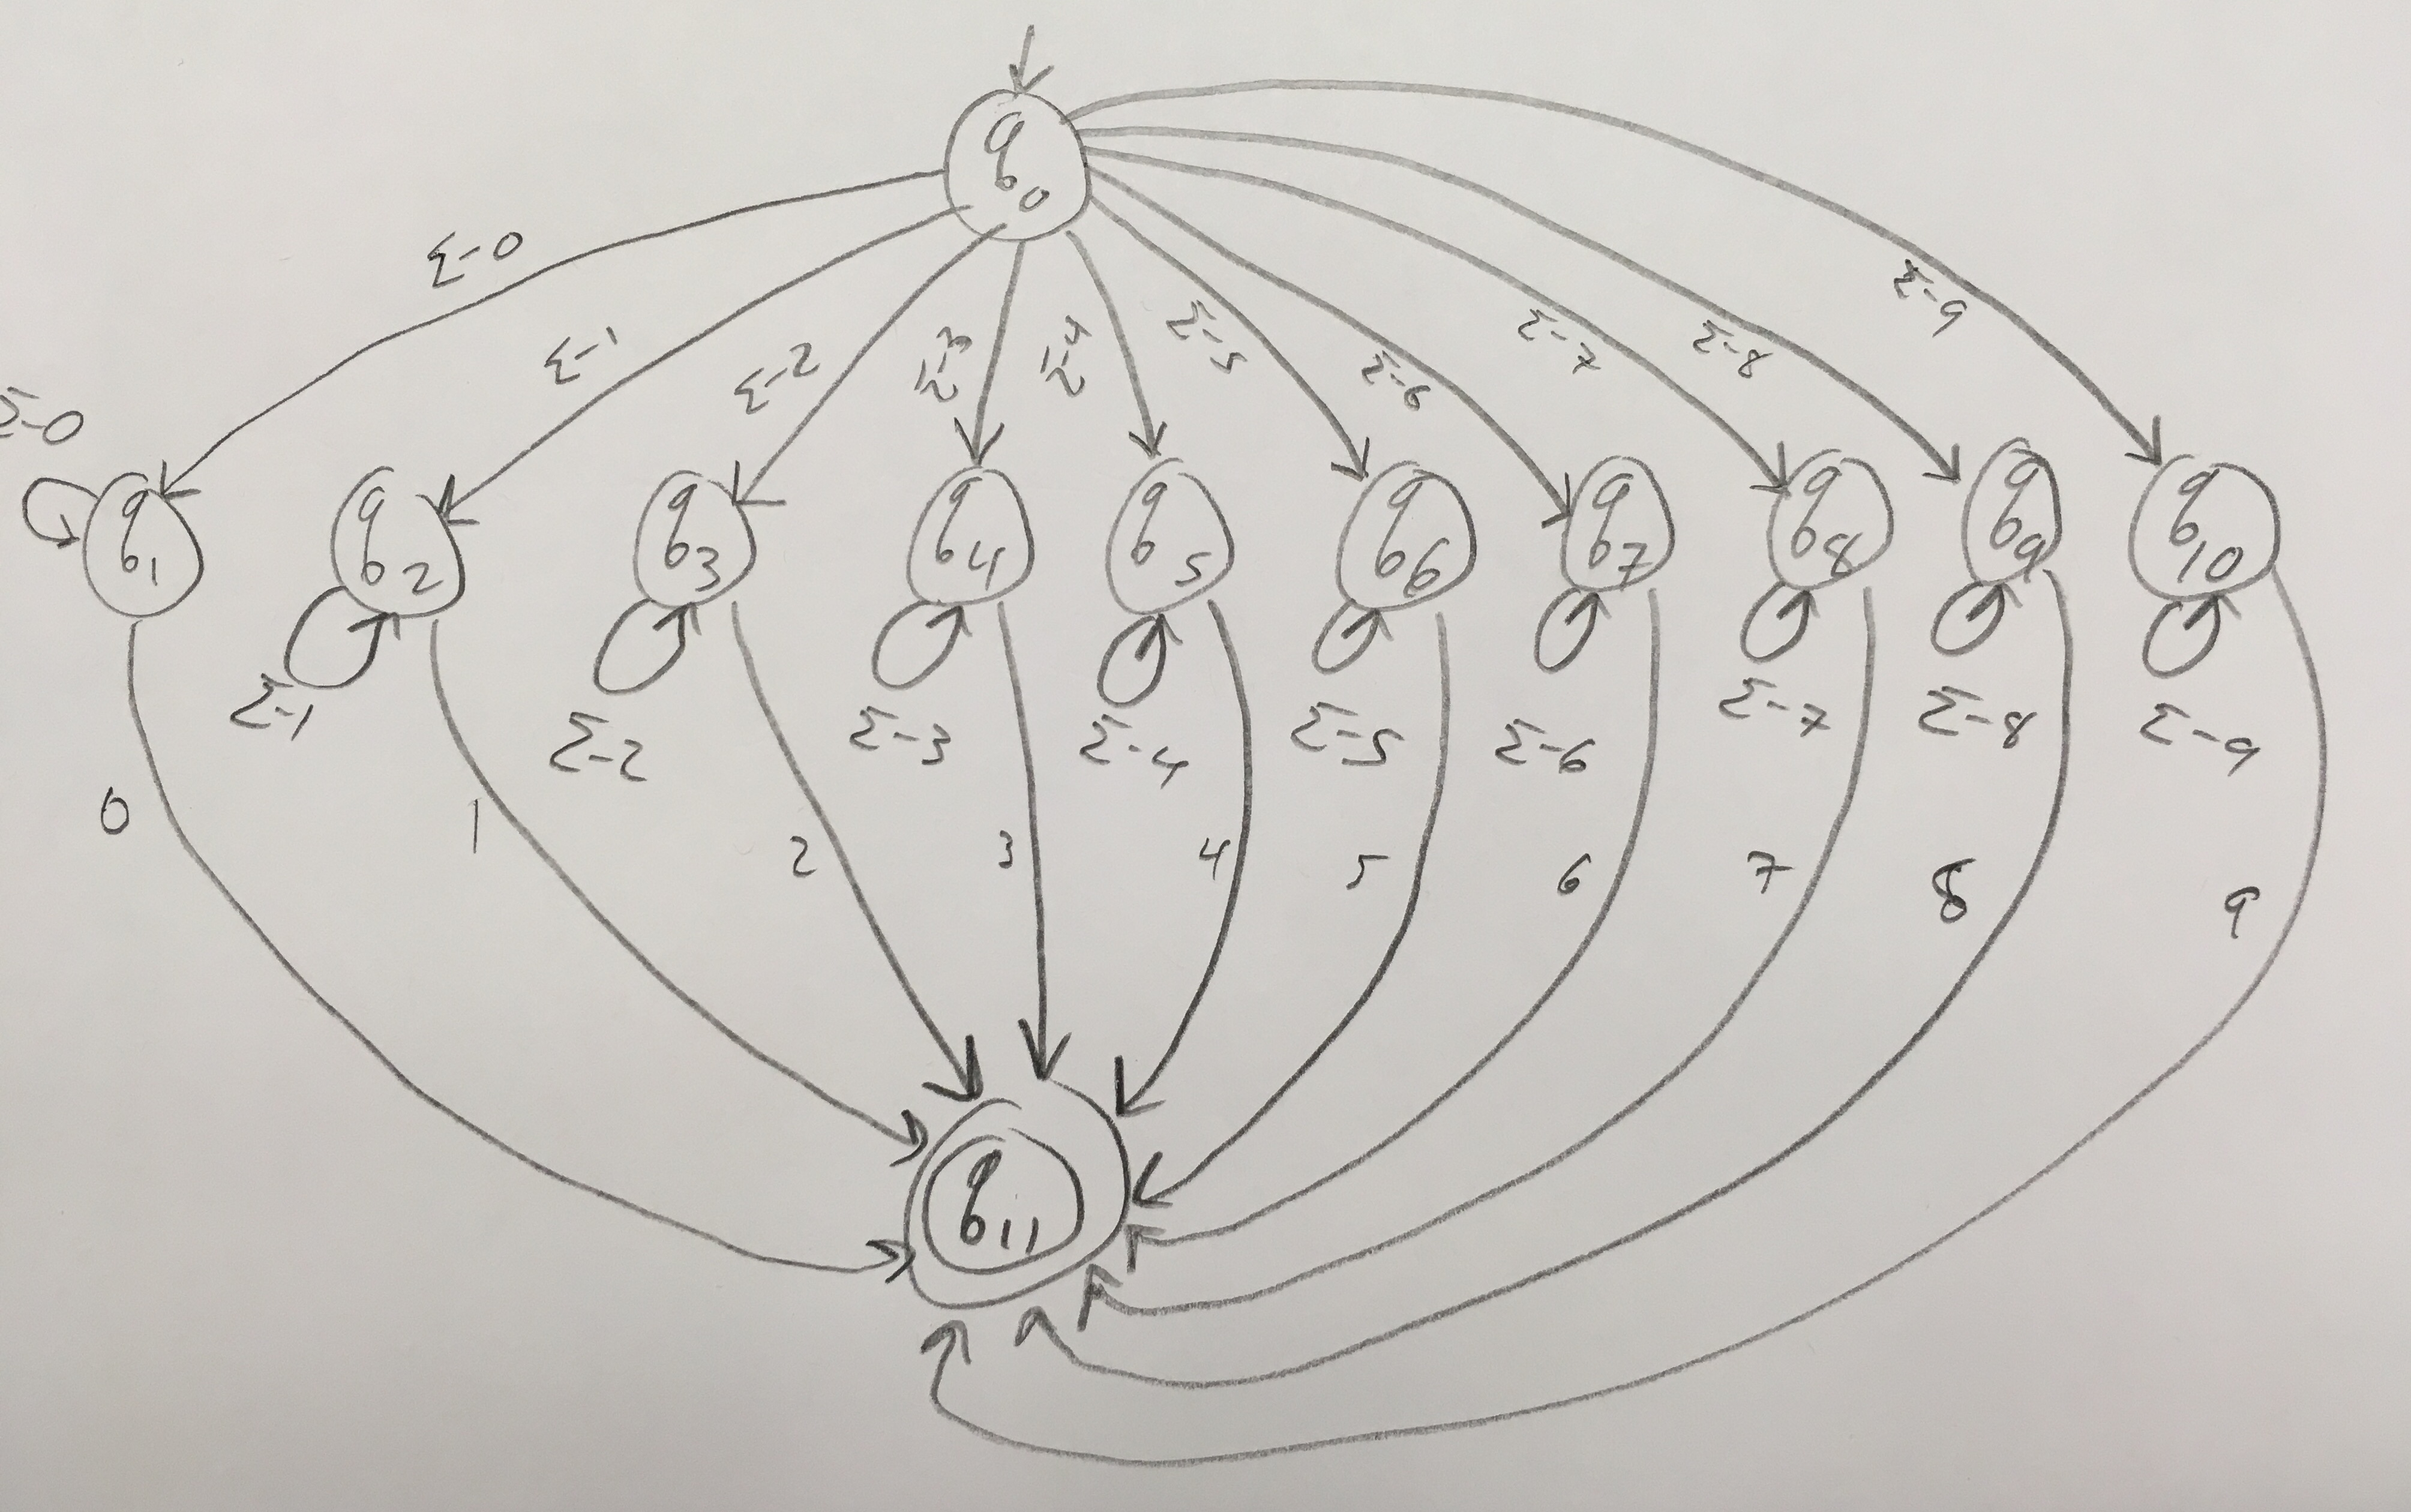
\includegraphics[width=\linewidth]{./figures/h2-4.jpg}
   	\end{subfigure}
\end{figure}
\subsection{c). The set of strings of 0's and 1's such that there are two 0's separated by a number of positions that is a multiple of 4. Note that 0 is an allowable multiple of 4}
\begin{figure}[!htbp]
  	\centering
   	\begin{subfigure}[p]{0.7\linewidth}
    	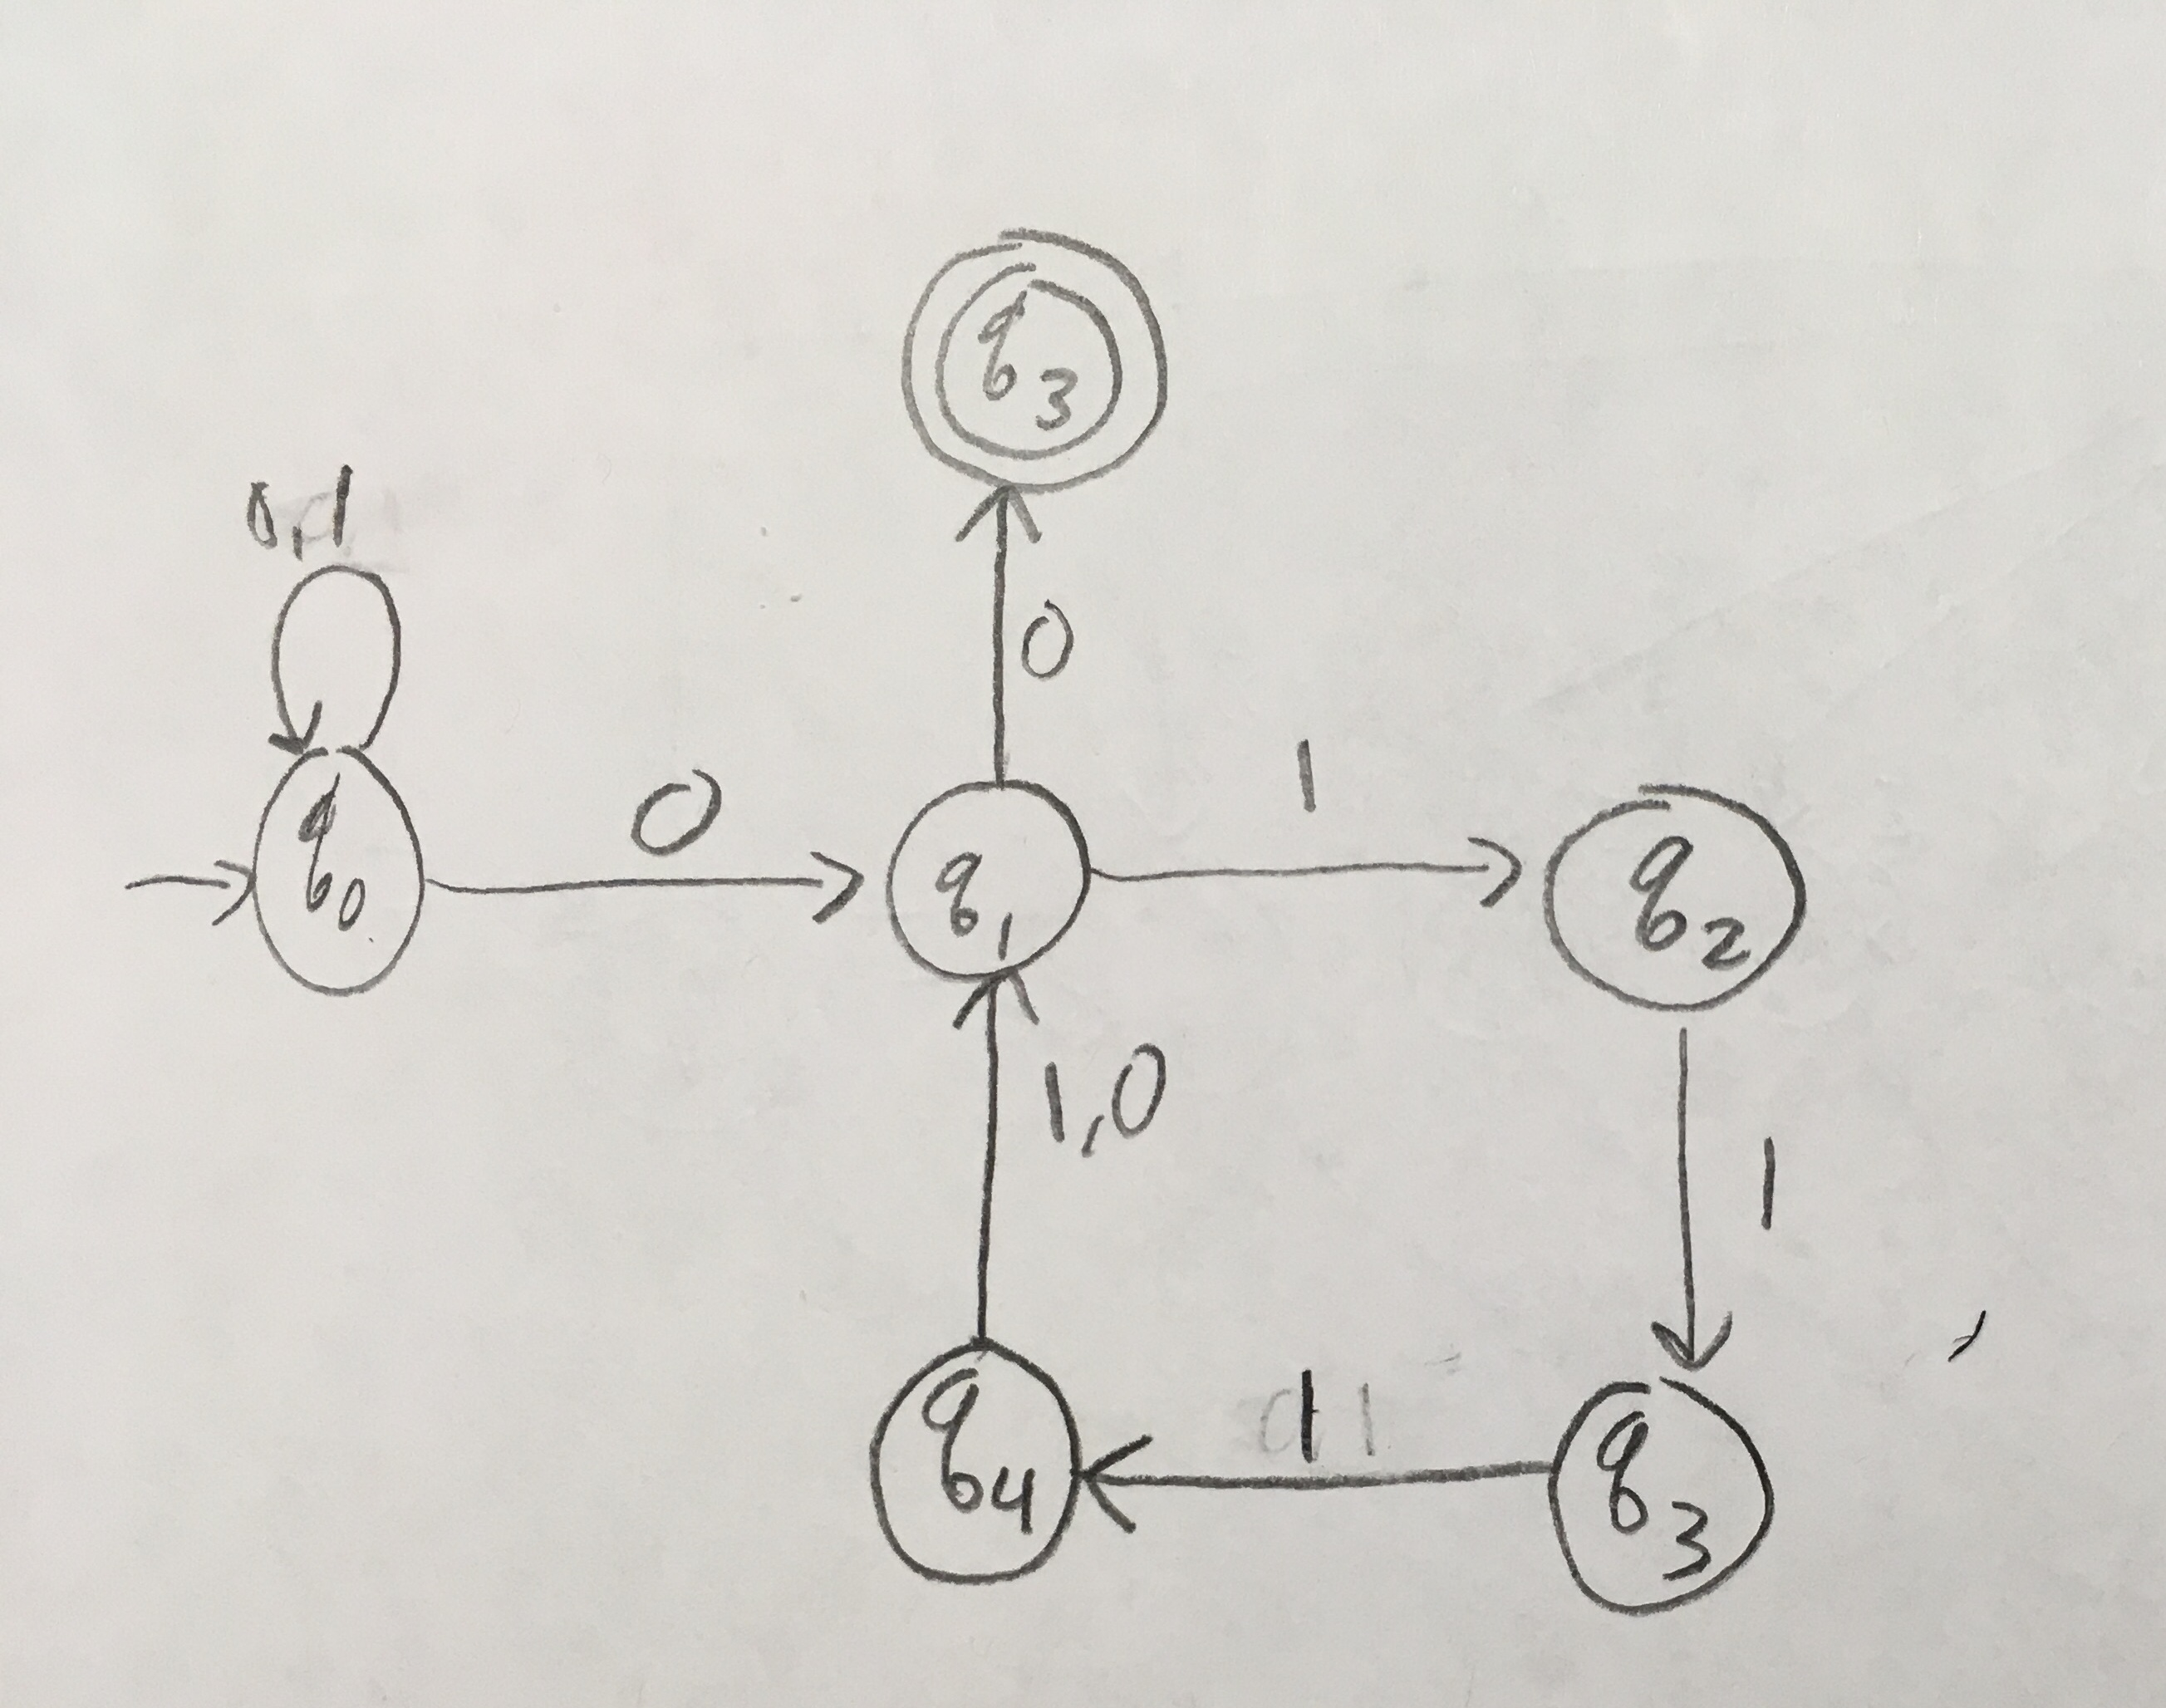
\includegraphics[width=\linewidth]{./figures/h2-5.jpg}
   	\end{subfigure}
\end{figure}


\section{Problem 2.4.1}
Design NFA's to recognize the following sets of strings:

\subsection{a). $abc$, $abd$, and $aacd$, Assume the alphabet is $\{a,b,c,d\}$.}

\subsection{b). $0101$, $101$, and $011$.}

\subsection{c). $ab$, $bc$, and $ca$. Assume the alphabet is $\{a,b,c\}$. }

\section{Problem 2.4.2b}
Convert each of your NFA's from Problem 2.4.1 to DFA's (We only complete part b here).
\noindent\rule{2cm}{0.4pt} \\


\end{document}
